\documentclass[12pt]{article}

\usepackage{graphicx} % Required for inserting images
\usepackage[margin=2cm]{geometry}
\usepackage{booktabs}
\usepackage{amsmath}
\usepackage{amssymb}

\usepackage{hyperref}
\urlstyle{same}

\graphicspath{{./images/}}

\title{Reading CAPTCHAs via Convolutional Neural Networks and Transfer Learning}
\date{}

\begin{document}

\maketitle

\section*{Introduction}

% Main objective of the analysis that also specifies whether your model will 
% be focused on a specific type of Deep Learning or Reinforcement Learning 
% algorithm and the benefits that your analysis brings to the business or 
% stakeholders of this data.

The CAPTHCA, or Completely Automated Public Turing test to tell Computers
and Humans Apart, was a common form of preventing automated bots from accessing
web applications. They generally consisted of a string of characters, typically
the latin alphabet and arabic numerals, printed in a non-standard format, either
by transforming the characters in some way or obsuring them with additional
marks. While this was common practice at one point, more sophisiticated methods
of distinguishing between humans and bots have since been implemented (e.g.
reCAPTCHA). However, some older repositories which no longer need to be
protected from automated access are no longer maintained and thus are still
locked behind the classic CAPTCHA test. To ease the access of this data, we can
train convolutional neural networks (CNNs) to read and recognize these
characters.

% Brief description of the data set you chose, a summary of its attributes, 
% and an outline of what you are trying to accomplish with this analysis.

The data set used here can be found in its entirety on Kaggle.com at
\url{https://www.kaggle.com/datasets/johnbergmann/captcha-image-dataset}. It
contains separate training and test sets of 8500 and 1500 CAPTCHA images,
respectively, with their correct labels in the file name for each image. The 
CAPTHCAs are greyscale JPEG images with a size of 50 $\times$ 250 pixels for a
total of 12,500 pixels, and each features 6 characters which is either a letter 
or a number. 

Because the format for each CAPTCHA is the same, we will develop six separate
models which will take the entire image and make a prediction for a single
character, rather than developing a single model that can take any CAPTCHA and
make a prediction, a significantly more complicated task. Additionally, because
each of the models will be a CNN which will be making similar predictions, we
can take advantage of transfer learning to speed up the training of subsequent
models.

\section*{Exploratory Data Analysis and Preprocessing}

% Brief summary of data exploration and actions taken for data cleaning or 
% feature engineering.

Only a small amount of feature engineering was necessary for the data set. Using
the \texttt{PIL} Python package, the images were converted to an array of pixel
values. Because all of the images are greyscale, the RBG tuple of each pixel
could be converted into a single value, resulting in a rank 4 array with the
dimension sizes $(n, 50, 250, 1)$, where $n$ is either 8500 or 1500 for the
train and test sets, respectively. Because we know that all of the images are
greyscale, we can format the samples to have a depth of 1, but it would be
simple to adapt this model to include all 3 channels of the original RGB pixel
values if a different data set was used. Finally, all of the array values were
divided by 255 to keep the inputs between 0 and 1.

The labels for each CAPTCHA were included in the filename for each image and
were recorded as the images were converted. These strings were all converted to
uppercase, as characters are in the CAPTCHA, and separated into their respective
characters to give an array of size $(n, 6)$ where each column corresponds to a
single character position. By using a single column of these labels, we can 
train a model to predict only that character position. Finally, each column was
one-hot-encoded using scikit-learn's \texttt{OneHotEncoder} to be used as
training output for each character position.

\section*{Model Training}

% Summary of training at least three variations of the Deep Learning model you
% selected. For example, you can use different clustering techniques or 
% different hyperparameters.

A simple CNN model was used as the base for the first set of models to test the
feasability of this method. The layers for this model are summarized below:

\begin{tabular}{ll}
    \toprule
	Layer        & Parameters \\
	\midrule
	Conv2D       & 32 filters, 5$\times$5 size, 2$\times$2 stride, ReLU
		activation  \\
	Conv2D       & 32 filters, 5$\times$5 size, 2$\times$2 stride, ReLU
		activation  \\
	MaxPooling2D & 2$\times$2 pooling size  \\
	Flatten      &   \\
	Dense        & 64 nodes, ReLU activation \\
	Dense        & 21 nodes, softmax activation \\
	\bottomrule
\end{tabular}

The models were compiled with a batch size of 64, 15 epochs and shuffling turned
on. With $\sim$400 thousand trainable parameters per model, each epoch took
between 17 and 20 seconds. Overall, the total accuracy for all predictions was 
$80.23\%$; however, the accuracy per label was only $39.60\%$. All six models
need to make correct predictions in order to produce the correct label. With an
average accuracy of $80\%$ for each model, that gives a probability of correctly
predicting the full label of approximately $26\%$. Here, we likely see better
performance because the labels with features which make prediction difficult
affect all of the models and will result in multiple errors for the same label.
Below is a heat map of the incorrect predictions which shows which pairs of
characters were likely to be confused. 

\begin{center}
	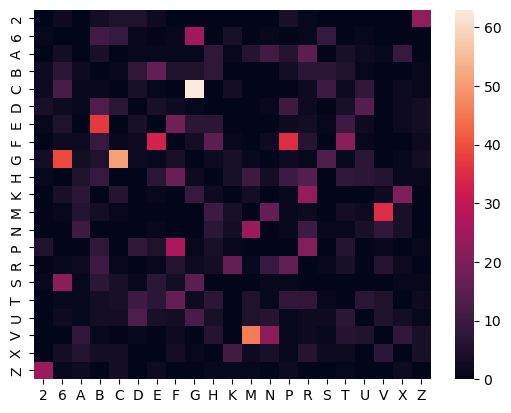
\includegraphics[width=3.5in]{heatmap1.png}
\end{center}

With the inital test showing promising results, a more complicated CNN was
implemented, this time taking advantage of transfer learning techniques. The
layers were split between feature layers which would be frozen between models
and the classification layers which would be trained separately for each model.
The summary for each layer is shown below:

\begin{tabular}{ll}
    \toprule
	Layer        & Parameters \\
	\midrule
	Feature Layers \\
	Conv2D       & 32 filters, 5$\times$5 size, 2$\times$2 stride, ReLU
		activation  \\
	Conv2D       & 32 filters, 5$\times$5 size, 2$\times$2 stride, ReLU
		activation  \\
	Conv2D       & 32 filters, 5$\times$5 size, 2$\times$2 stride, ReLU
		activation  \\
	MaxPooling2D & 2$\times$2 pooling size  \\
	Dropout      & 0.25 dropout rate \\
	Flatten      &   \\
	\\
	Classification Layers \\
	Dense        & 512 nodes, ReLU activation \\
	Dropout      & 0.25 dropout rate \\
	Dense        & 256 nodes, ReLU activation \\
	Dense        & 21 nodes, softmax activation \\
	\bottomrule
\end{tabular}

After the first model was trained, the feature layers were frozen and used to
train the subsequent models. With 975 thousand trainable parameters, the first
model took 15 to 19 seconds per epoch, but for the following models each epoch
only took 3 to 5 seconds, significantly speeding up the training process.
Unfortunatly, the additional layers only resulted in a moderate increase in
performance with a character accuracy of $82.02\%$ and a label accuracy of
$41.00\%$. 

The next step to improving the performance of the models is to allow for fine
tuning of the models. After allowing the subsequent models to undergo transfer
learning for 10 epochs, the feature layers are unfrozen for 5 more epochs and
allowed to adjust their parameters for the specfic characters they are 
analyzing. Doing so slightly improves the performance for a character accuracy
of $85.33\%$ and a label accuracy of $45.73\%$. 

% A paragraph explaining which of your Deep Learning models you recommend as a
% final model that best fits your needs in terms of accuracy or explainability.

The final model which utilizes both transfer learning as well as fine tuning
provides the best performance with considerable time cost savings. While the
models here would only succeed about half of the time, a single prediction takes
fractions of a second, the two or three attempts needed to succeed could be
accomplised before a human could fully register what the first character.

\section*{Summary}

% Summary Key Findings and Insights, which walks your reader through the main 
% findings of your modeling exercise

We were able to develop a series of models which could predict the correct label
for a CAPTCHA for approximately $45\%$ of attempts. While this may seem low,
several attempts can be made considerably faster than a human could make a
single attempt. In these various models, we saw that transfer learning was very
success at reducing the time needed for training, reducing the time for a single
epoch to a fourth of the original time. Fine tuning was also helpful in teasing
out a small additional boost to the character and label accuracy of the models.
Becuase the CAPTCHAs are fairly inconsistent by design, it helps to have the
models for each character have the chance to adjust their feature layers to suit
the individual characters.

% Suggestions for next steps in analyzing this data, which may include 
% suggesting revisiting this model or adding specific data features to achieve
% a better model.

The easiest way to improve the models would be to increase the number of layers 
present in either the feature layers or the classification layers. The CAPTCHAs 
feature a variety of different tricks for obscuring the characters, and the 
previous heat map showed how the most similar characters were confused (e.g. 6 
and G). To further distinguish between these characters, a more sophisticated 
model is needed to discover the unseen latent features.

\end{document}
